\section{Constraint Episode Mining and Mixture EGH}
We use a two-pronged approach to tackle the problem of mining and predicting unoccupancy.
First, we use an episode mining algorithm to discover frequent events before a person leaves 
a room. Then we use a mixture HMM model, EGH, to predict whether the room is unoccupied
and when the person leaves and comes back. 
%Then the possible time of the prediction  event will be predicted by averaging the past time. 

\subsection{Time-gap Constraint Episode Mining}
Episode mining has been studied in previous research \cite{mannila1997discovery} 
and \cite{laxman2005discovering}. 
Assume there is an event stream $s=ACBDEDEAABBA$, 
and the target episode is $AB$. To mine for $AB$, we can can use non-overlap mining approach to find the target episode. 
Non-overlap mining can be used where any two instances of the target episode has no intersection. It is to be noted that, non-overlap episode mining may result in different instances. 
For instance in the above example, if we align it to the left,  the episode mining results are $\langle A_1, B_3 \rangle, \langle A_8,B_{10} \rangle$. If aligned to the right, the results become as $\langle A_1, B_3 \rangle, \langle A_9,B_{11} \rangle$. 
A variant of episode mining is event gap constraint episode mining as proposed in
\cite{patnaik2008inferring}. 

In this application, 
the events dwell at an event for a period of time. 
Therefore, we combine the above two 
episode mining algorithms and enforce more constraints.
The first change is to 
use the right alignment for the first element in the episode. 
In the example of $AB$, 
the mined second instances is $\langle A_9,B_{11} \rangle$. 
The second modification is to 
check the time constraints and 
apply gap duration constraints between 
two consecutive events inside an episode. 
Figure \ref{fig_durationgapconstraint} shows an example of time-gap constraint episode. 
\begin{figure}[h]
\centering
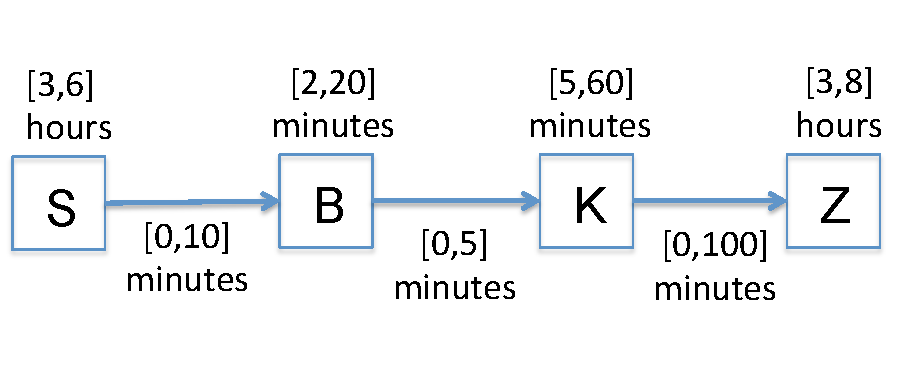
\includegraphics[width=0.7\textwidth]{adlfigs/durationgapconstraint.pdf}
\caption{Example of Duration-gap Constraint Episode.\label{fig_durationgapconstraint}}
\end{figure}

Assume we have the frequent episode $S\rightarrow B \rightarrow K\rightarrow Z$, 
we add the time constraints to each event $\{S,B,K,Z\}$. 
The dwelling duration of $S$ is 3 to 6 hours,   
of $B$ is 2 to 20 minutes, 
of $K$ is 5 to 60 minutes, 
and of $Z$ is 3-9 hours. 
Also, we set gap duration between any two consecutive events. 
The gap duration of $SB$ is calculated as $\Delta{SB} = B.start - A.end$. 
We set the maxim gap time between SB, BK, and KZ as 
10 minutes, 5 minutes and 100 minutes; 
the minimal gap time is 0. 
Figure \ref{fig_MingExample} is a time-gap constraint episode mining example. 
We have a stream composed of a sequence of dwelling events and the target 
episode is the same as in Figure \ref{fig_durationgapconstraint}.
The unit of the figures is in minutes.  
\begin{figure}[!hbtp]
\centering
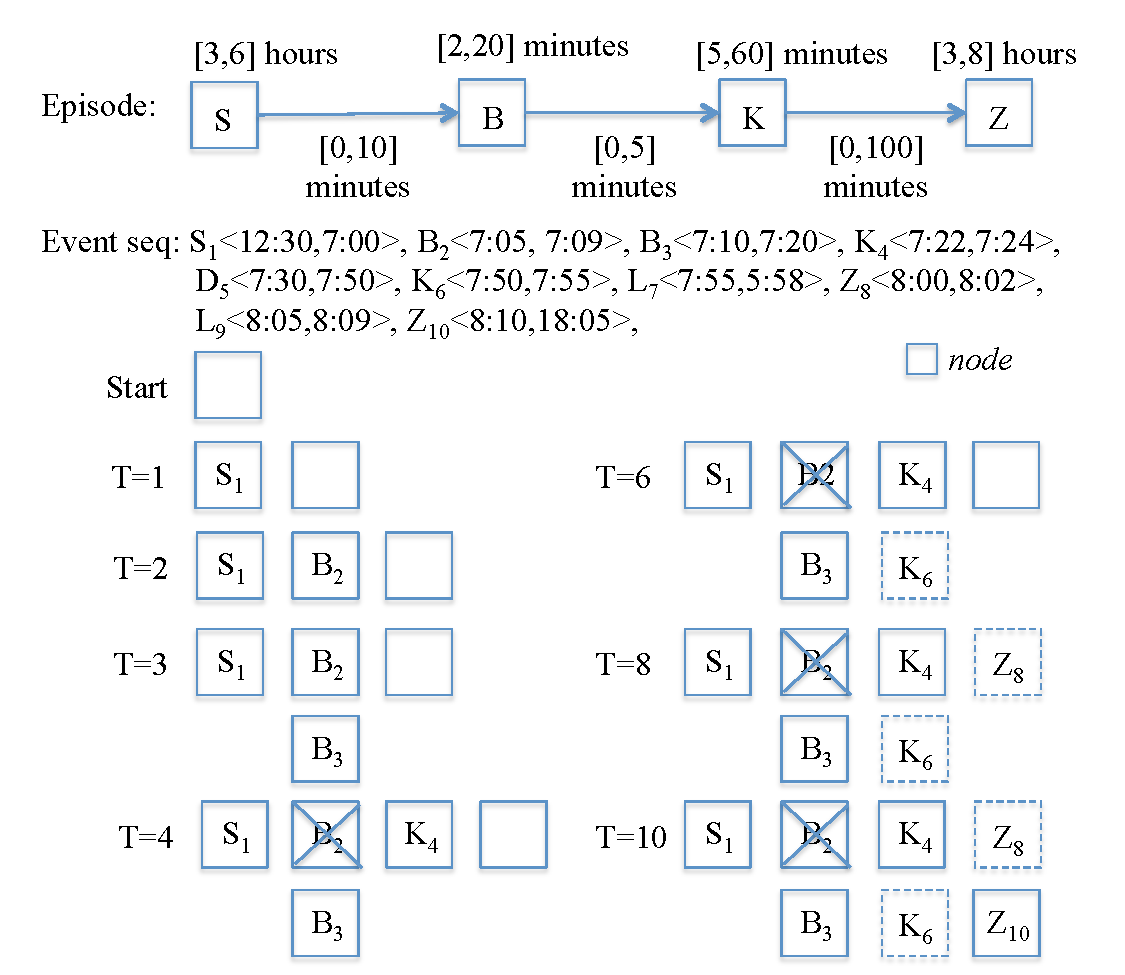
\includegraphics[width=1.0\textwidth]{adlfigs/MingExample.pdf}
\caption{Time-gap constraint episode mining example.\label{fig_MingExample}}
\end{figure}

Initially, a $waits$ structure related to this episode is created. 
Each $waits$ structure has the same length of episode structure $node$. 
A $node$ structure related to $S$ is created 
and it waits for the first 
element of the episode $S\langle 180, 360 \rangle $. 
When $T=1$, the duration of $S1$ is checked. 
Since it's in the range of $3-6$ hours, 
$S1$ passes and is put into the node structure $node$ related to $S$. 
Then a new $node$ structure is created to wait for $B\langle 2, 20 \rangle $. 
When $T=2$ and $T=3$, both of the $B2$ and $B3$ 
are qualified in terms of the time constraints and 
the gap constraints, 
e.g. the gap between $S$ and $B$ $\Delta SB$ should 
be between 0 to 10 minutes. 
Then $B2$ and $B3$ are input into the $node$ $B$ structure in the 
$waits$ structure. 
At the same time, 
a new $node$ structure is created for $K\langle 5, 60 \rangle $. 
When $T=4$, the gap between $\langle B3, K4 \rangle$ 
is satisfied with the distance condition between 
$B$ and $K$ 0-5 minutes. 
But the gap between $\langle B2, K4 \rangle$ 
is longer than the constraint gap. 
Therefore, $B2$ is canceled off. 
Now a new $node$ waits for the symbol $Z\langle 180, 540 \rangle$. 
When $T=6$, the gap from $B2$ and $K6$ is 
too far. Therefore, $K6$ is not added into the $node$ $K$ structure in $waits$.
When $T=8$, the time duration of $Z8$ is not qualified the condition between 3-9 hours. 
$Z8$ is not added. 
When $T=10$, the duration of $Z10$ meets the requirement 3-9 hours 
and its distance to $K4$ meet the requirement 
of $\Delta KZ \in [0,100]$ minutes. 
Thus $Z10$ is added into the $node$ $Z$ structure in $waits$.
Therefore, a complete episode mining is done. 

This complete gap-constraint episode mining on dwelling events 
is described in detail in Algorithm \ref{alg_episodeMiningConstraint}
%\ref{alg_episodeMiningConstraint_2e} 
in the appendix section.

%Non-overlap episode mining is defined as \textit{Definition}. 

\subsection{Episode Generating HMM}
Each frequent episode is connected with an HMM. 
According to EGH \cite{laxman2005discovering}, 
each episode generated HMM 
only has a noise parameter $\eta$.
The noise parameter $\eta$ of frequent episode $\alpha$ 
is calculated as $\eta=\frac{T-Nf_{\alpha}}{T}$ \cite{laxman2005discovering},  
where $T$ is the training data stream length, 
$\alpha$ is the frequent episode, 
$N$ is the length of frequent episode $\alpha$, 
$f_{\alpha}$ is the frequency over the time $T$.

Figure \ref{fig_egh} gives an example of the transition matrix in EGH. 
Assume we have a N-node frequent episode $S\rightarrow B\rightarrow Z$ and $N=3$ here.
We define 2N number of hidden states, 
N for episode states, and N for noise states. 
The noise states are $W\rightarrow X \rightarrow Y$. 
An episode state transfers to another episode state 
at the probability of $1-\eta$.
An episode state transfers to a noise state 
at a probability of $\eta$. 
A noise state transfers to another noise state 
at a probability of $1-\eta$. 
The emission matrix is calculated as following. 
Let M denote the totally number of symbols in the event stream. 
For any hidden states in the episode, it has a delta function emission. 
Whenever it is visited (right alignment of the first element in the episode, 
left alignment for the left elements in the episode), 
it will generate the same observation symbol. 
For any noise hidden states, it emits any of the symbols from the $M$ 
observation symbols with a uniform distribution at probability $\frac{1}{M}$. 

\begin{figure}[!hbtp]
\centering
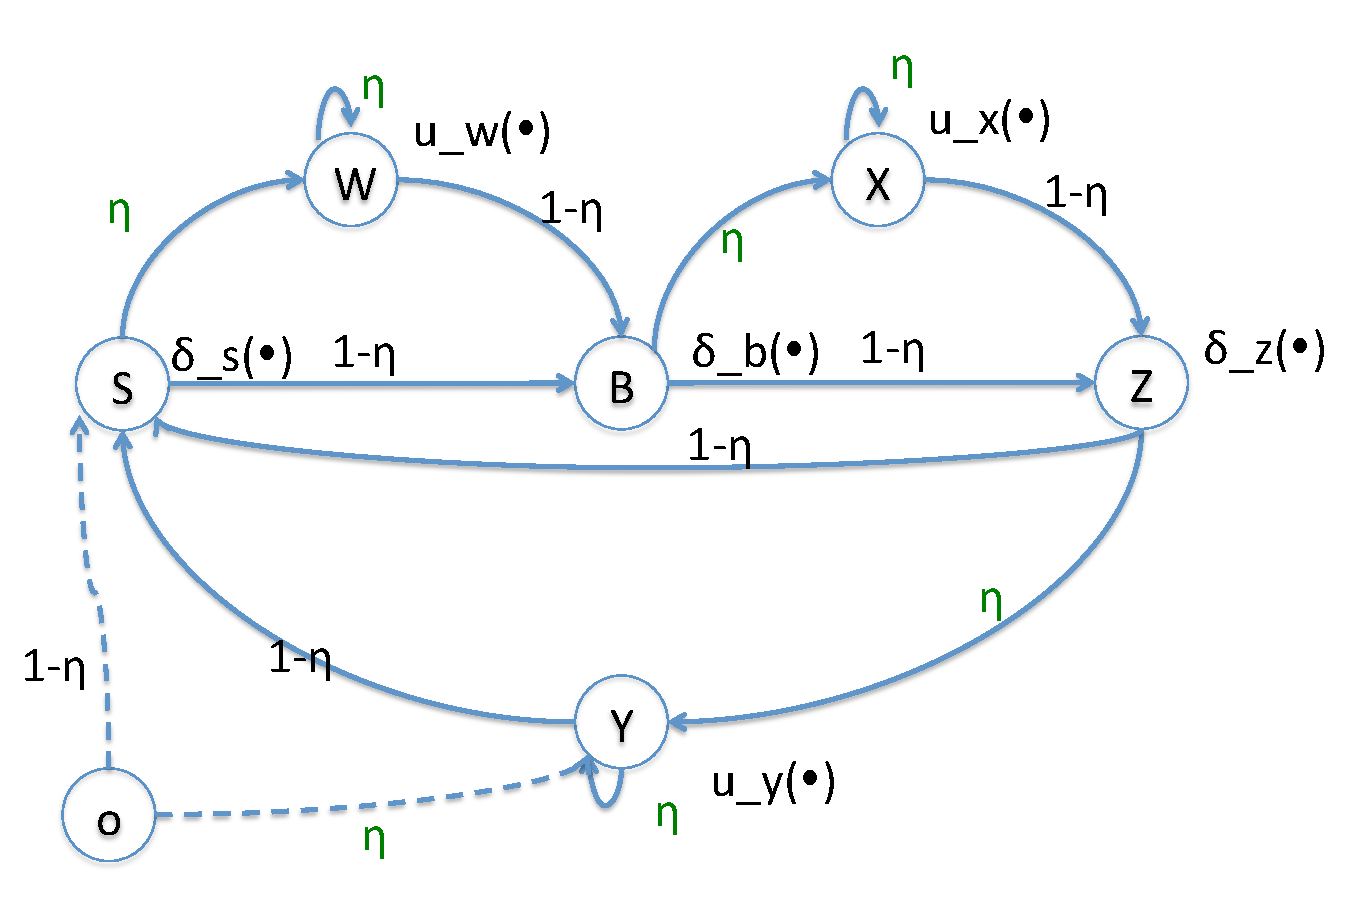
\includegraphics[width=0.7\textwidth]{adlfigs/egh.pdf}
\caption{States Transition of Episode Generating HMM (EGH).\label{fig_egh}}
\end{figure}


Theorem \ref{theorem1}~\cite{laxman2005discovering} is very important. 
It guarantees that the more frequent an episode inside the sequence, 
the probability of most likely sequence is larger. 
Its proof is explained in detail in \cite{laxman2005discovering}. 


\newtheorem{mydef}{THEOREM}
\begin{mydef}
\label{theorem1}~\cite{laxman2005discovering} 
Let $D_Z={X_1,..., X_K}$ is the given sequence data,  $\varepsilon$ is the symbol set, 
and the size of these symbols is $M$. 
Given two frequent N-node episodes $\alpha$ and $\beta$ with frequency $f_{\alpha}$ 
and $f_{\beta}$. Their corresponding EGH is $\Lambda_{\alpha}$ and $\Lambda_{\beta}$. 
The most likely state sequence for episode $\alpha$ and $\beta$ are
$q_{\alpha}^*$ and $q_{\beta}^*$. 
The noise parameters of these two EGH are 
$\eta_{\alpha}$ and $\eta_{\beta}$. 
Assume both of these noise parameters are less than $\frac{M}{M+1}$, 
we have 
(1) if $f_{\alpha} > f_{\beta}$, the $P(D_Z, q_{\alpha}^*| \Lambda) > P(D_Z, q_{\beta}^*| \Lambda)  $
(2) if $P(D_Z, q_{\alpha}^*| \Lambda) > P(D_Z, q_{\beta}^*| \Lambda)  $, $f_{\alpha} > f_{\beta}$
\end{mydef}

In this occupancy prediction application, 
we change the calculation of frequency. 
In our work, the frequency of episode 
is based on day. 
If an episode happens more than once, 
then we calculate it as only once. 

\subsection{Mixture EGH}
Mixture EGH has been discussed fully in previous work \cite{laxman2005discovering}.
The mixture EGH model has the advantage of 
giving different weight for each EGH model
for prediction. 
From the previous subsection, 
we obtain whether an episode occurs in a certain day. 
Let $D_Z=\{X_1,..., X_K\}$ denote the $K$ days data set. 
$F=\{\alpha_1, ... \alpha_J\}$ denote the frequent episodes in the dataset $D_Z$. 
EGH $\Lambda_{\alpha_j}$ 
corresponds to 
one of the frequent episode $\alpha_j$.
Let $\Lambda_Z$ denote the mixture model. 
The likelihood of $D_Z$ under the mixture model is written as Equation \ref{eq_mixture}.
\begin{eqnarray}
\label{eq_mixture}
Pr(\Lambda|Z) &=& \prod_{i=1}^K P[X_i|\Lambda_Z] \\
			&=& \prod_{i=1}^K ( \sum_{j=1}^J \theta_j P[X_i| \Lambda_{\alpha_j}])
\end{eqnarray}
where $\theta_j$ is the mixture coefficient of $\Lambda_{\alpha_j}$ and it subjects to 
$\sum_{j=0}^J \theta_j=1$ 

The parts inside Equation \ref{eq_mixture} are additive, 
the coefficients $\theta$ are computed by EM algorithm. 
The detailed description is algorithm %%%\ref{alg3} 
in the 
appendix section.
%% algorithm 03
\renewcommand{\algorithmicrequire}{\textbf{Input:}}
\renewcommand{\algorithmicensure}{\textbf{Output:}}

\begin{algorithm}
\caption{EM Algorithm for mixture EGH}
\label{alg3}
\begin{algorithmic} [1]
\REQUIRE day episode matrix, 
each element $e_{ij}$ records for each day whether an episode $j$ happens in day $i$;
frequent episodes $F=\{\alpha_1, ..., \alpha_J\}$;
symbol set $\varepsilon$;
threshold $\gamma$

\ENSURE the parameters for mixture EGH $\Lambda_Z=\{  (\Lambda_{\alpha_j}, \theta_j ) , j=1,...,J \}$


\STATE calculate the number of episodes J, and number of days K
\STATE calculate all $\eta$s' threshold value $mThreshold= \frac{M}{M+1}$

\COMMENT{initialize all the thetas to be $\frac{1}{J}$}
\COMMENT{calculate the total frequency for each episode over training time series}
\COMMENT{ calculate the $eta$ value}
\FOR{$0 \leq j \leq J$}
\STATE $\theta[j]= 1/J$
\STATE $episodeFreq[j] = \sum_i^K e_{ij}$
\ENDFOR

\STATE select those frequent episodes starting with 'S' and ending with 'Z' and separate these 
episodes by workday or holiday

\COMMENT {calculate $eta$ for each episode} 
\FOR{$0 \leq j \leq J$}
\STATE $\eta[j]= 1-episodeLen[j]*episodeLen/T$
\ENDFOR

\COMMENT{likelihood prediction of each episode $j$ in the $k$th day}

\FOR{$0 \leq i \leq K$}
\FOR{$0 \leq j \leq J$}
\STATE $likelihood_{ij} = \frac{1-\eta[j]}{\eta[j]/M} ^ {episodeLen[j]*e_{ij}}$
\ENDFOR
\ENDFOR

\COMMENT{calculate the obj value based on J, K, $likelihood_{ij}$ and $\theta$}
\WHILE{$newObj- obj > \gamma$}
\STATE $\theta_{new}=[]$
\FOR{$0 \le l \le J$}
\STATE $temp=0$
\FOR{$0 \le j \le K$}
%\COMMENT{calcuate the new likelihood with Bayes rules}
\STATE $temp = temp+ \frac{\theta_l*likelihood_{il}}{ \sum_0^J { \theta_j*likelihood_{ij}}}$

\ENDFOR
\STATE $\theta_{new}[l] = temp/K $
\ENDFOR

\STATE calculate the newObj
\IF{$newObj-obj > \gamma$}
\STATE $obj=newObj$
\STATE $\theta_{new} = \theta$
\ENDIF

\ENDWHILE

\STATE Output $\Lambda_Z=\{  (\Lambda_{\alpha_j}, \theta_j ) , j=1,...,J \}$

\end{algorithmic}
\end{algorithm}
During the initialization %line 1-10
part of the EM algorithm, 
the episode frequency over the times series T is calculated. 
Specific frequent episodes ended with target event 'Z' are selected. 
Optionally, 
we could add special constraints on episodes starting with 
certain event type 'S'. 
%calculated in lines 11-16. 
In the expectation step, 
one key part is the likelihood value of each episode $\alpha_j$ in time series $X_i$.
The likelihood value is computed as Equation \ref{eq_likelihood}.
Then Bayes rules is applied to compute the new coefficient $\theta_{new}$. 
\begin{equation}
\label{eq_likelihood}
Pr(X_i| \Lambda_{\alpha_j}) = (\frac{\eta_{\alpha_j}}{M})^{|X_i|} (\frac{1-\eta_{\alpha_j}}{\eta_{\alpha_j}/M})^{|\alpha_j|f_{\alpha_j}(X_i)}
\end{equation}
In the step of maximization, 
we can update the objective value based on Equation \ref{eq_mixture}. 
and until it converges, i.e., 
the difference of two consecutive objective values 
is smaller than a threshold.%$\gamma$.

\subsection{Predict When the Target Event Occurs}
Target event prediction has been studied in  \cite{laxman2008stream}. 
But it only predicts whether a target event will occur or not. 
It never considers when the target event will happen. 
The occupancy prediction problem involves three sub-problems: 
1) whether the target event un-occupancy $Z$ will appear; 
2) when the target event $Z$ starts; 
3) when the target event $Z$ ends. 

For stream prediction for target event, 
refer to algorithm in \cite{laxman2008stream}. 
This section emphasizes on the last two sub-problems, 
predicting when the person leaves  $Z_{leave}$ or comes back $Z_{back}$ 
after we already know target event $Z$ will surely happen. 
Note that $Z_{leave}$ corresponds to $Z.start$, when the $Z$ event starts. 
$Z_{leave}$ corresponds to $Z.end$, when the $Z$ event ends. 
This prediction algorithm is described in algorithm \ref{alg22}. 

After running episode mining and mixture EGH model, 
we have obtained all the frequent episodes $F=\langle \alpha_1,..., \alpha_J \rangle$, 
the corresponding EGH $\Lambda_{\alpha_j}, j=1...J$ with noise parameter $\eta_j$, 
and the mixture models $\Lambda_Z$ with coefficients $\theta_j$.
We use the coefficient of these mixture models for leave time and back time prediction. 
The algorithm \ref{alg22} 
uses partial day of test data $s$, 
all the frequent episodes  $epis$, 
the frequent episodes $F$ in partial day of $s$, 
the mixture model $\Lambda_Z$, 
to predict when the person leaves or comes back home. 
The partial day is cut by partial index $pIndex$. 
Each day is cut into three phases, before the person gets up; 
after the person gets up but before the person leaves home;
after the person comes back home. 

In the first two phases, before the person leaves, 
the PDF leave time and back time are calculated from line 2-4. 
Usually before a person gets up, there is only one frequent episode named 'SZ'. 
After the person gets up, he/she has a lot of activities at home, 
there are several frequent episodes mined before the person leaves home. 
In case there are several frequent episodes in lines 6-12, 
the leave time and back time of each episode is checked
whether they are in a range of PDF value in the past. 
If yes, the mean value of these episodes are recorded from line 14-17. 
If there are several frequent episodes with corresponding EGH, 
the leave time $Z_{leave}$ and back time $Z_{back}$ is the weighted 
mean leave time and back time of each episode in lines 18-21. 

In the third phase, after the person leaves home, 
we already know when the person leaves home $Z_{leave}$ 
but needs to predict when the person comes back $Z_{back}$. 
If the person has come back, that means $Z_{back}$ is not equal to $Z_{leave}$. 
We don't need to do anything. 
If the person has not come back, that means $Z_{back}$ equals to $Z_{leave}$. 
The back time is the past weighted back time from line 28-34. 

% algorithm 22, an extention of algorithm 2
\renewcommand{\algorithmicrequire}{\textbf{Input:}}
\renewcommand{\algorithmicensure}{\textbf{Output:}}

\begin{algorithm}
\caption{ Target Event Occurs Time Prediction Algorithm}
\label{alg22}
\begin{algorithmic} [1]
\REQUIRE 
partial day cut point $pIndex$, $s[1:pIndex]$ is known,  and $s[pIndex:96]$ for prediction;
partial day event stream $s=\langle E_1,..., E_{pIndex} \rangle$;
all the episodes $epis$, $\forall E \in \alpha$ and $\forall \alpha \in epis$, E has $E.{start}$ 
and $E.{end}$; 
frequent episodes $F=\langle \alpha_1,..., \alpha_J \rangle$ inside $s[1:pIndex]$;
EGH model $\Lambda_{\alpha_j}$ with noise parameter $\eta_j$ where $j=1...J$
EGH mixture model coefficients $\Theta=\langle \theta_1,...,\theta_J \rangle$;
the slot number noise parameter $\epsilon$  ; 
target event $Z$
\ENSURE Predict target event leaving time $Z_{leave}$ and back time $Z_{back}$
 
\IF{$Z  \notin s $}%\COMMENT{predict before the person leaves home}
\STATE choose episodes $\alpha.ev={'SZ'}$ 
\STATE $Z_{leave} = \frac{\sum_1^K Z.start}{|\alpha|} $
\STATE $Z_{back} = \frac{\sum_1^K  Z.end}{|\alpha|}  $
\IF{$len(F)>1$}%\COMMENT{if there are several episodes to predict 'Z'}
\FOR{$\alpha_j \langle e_1,..., e_j \rangle \in F$}
%\IF{$\alpha_j.ev='SZ'$} % 'SZ' has been calculated,no need to calculate again
%\STATE break
%\ENDIF
\IF{$pIndex \in ( \alpha_j. ev[-2].start - \epsilon, \alpha_j.ev[-2].start+ \epsilon )$}
\STATE $leaveMap[\alpha_j.ev]=\alpha_j.leave$
\ENDIF
\IF{$pIndex \in ( \alpha_j. ev[-2].end - \epsilon, \alpha_j.ev[-2].end+ \epsilon )$}
\STATE $backMap[\alpha_j.ev]=\alpha_j.back$
\ENDIF 
\ENDFOR
\IF{$len(leavingMap) !=0 $} % for the average
\STATE $leaveSlotMap[\alpha_j.ev] =\frac{\sum_1^K leavingMap.get(k)}{K}$
\STATE $backSlotMap[\alpha_j.ev] = \frac{\sum_1^K backMap.get(k)}{K}$
\ENDIF % this is for the len\\
\IF{$K=len(leaveSlotMap)>1$}%\COMMENT{There are other frequent episodes except 'SZ'}
\STATE $Z_{leave}= \frac { \sum_{k=1}^K leaveSlotMap.get(k) * \theta_k } {K}$
\STATE $Z_{back}= \frac { \sum_{k=1}^K backSlotMap.get(k) * \theta_k } {K}$
\ENDIF
\ENDIF %this is for len(F)>1 
\ENDIF %this is for if Z \notin S \\
\IF{$Z  \in s $}%\COMMENT{if the person has left home}
\STATE $Z_{leave}=s.firstindex[Z]$ % the position where $Z$ first appears
\STATE $Z_{back}=s.lastindex[Z]$ % the position when $Z$ lastly appears\\
%\STATE backSlotMap=\{\}
\IF{$Z_{leave}=Z_{back}$} %\COMMENT{The person hasn't come back}% the person hasn't come back
% get the average of those time
\FOR{$\alpha_j \langle e_1,..., e_j \rangle \in F$}
\IF{$Z_{leave} \in [\alpha_j.ev[-2].end - \epsilon, \alpha_j.ev[-2].end + \epsilon ]$}
\STATE $backSlotMap[\alpha_j.ev] = \alpha_j.leave$
\ENDIF
\ENDFOR
\STATE $Z_{back}= \frac { \sum_{k=1}^K backSlotMap.get(k) * \theta_k } {K}$
\ENDIF
\ENDIF
\STATE Output the slot number when the person leaves $Z_{leave}$ and comes back $Z_{back}$
\end{algorithmic}
\end{algorithm}
 





